\begin{figure}[htbp]
    \pgfmathsetmacro{\xmin}{0.5}
    \pgfmathsetmacro{\xmax}{8.5}
    \pgfmathsetmacro{\ymin}{.5}
    \pgfmathsetmacro{\ymax}{6.5}
       \begin{subfigure}[b]{0.48\textwidth}
        \centering
        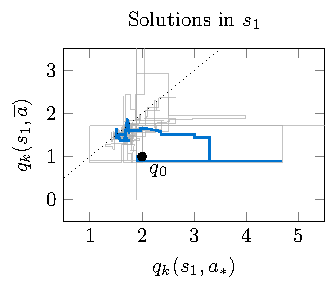
\includegraphics{figures/iv-simulation.pdf}
        % \begin{tikzpicture}[scale=1]
        %     \begin{axis}[
        %         xlabel={$q_k(s_1, \best{a})$},
        %         ylabel={$q_k(s_1, \worst{a})$},
        %         xmin=0.5, xmax=5.5,
        %         ymin=-0.5, ymax=3.5,
        %         xtick={1,2,...,5},
        %         ytick={0,1,2,...,3},
        %         title={Solutions in $s_1$},
        %         grid=none,
        %         % tick label style={font=\small},
        %         % label style={font=\small},
        %         width=0.9\linewidth,
        %         height=4.5cm,
        %     ]
        %         \pgfplotstableread[col sep=tab]{figures/33/3s_phase_st_s1.txt}\datatable
            
        %         \foreach \n in {1,...,9} {
        %             \pgfmathsetmacro\yindex{10+\n}
        %             \addplot [mygrey, opacity=0.7] table [x index=\n, y index=\yindex] {\datatable};
        %         }
        %         \addplot [CambridgeCoreBlue, line width=0.8pt] table [x index=0, y index=10] {\datatable};

        %         \addplot[color=black, mark=*, mark size=2pt] coordinates {(2, 1)};
        %         \node[text=black, below right] at (axis cs:2, 1) {$q_0$};
                
        %         \addplot[color=black, dotted, domain=\xmin:\xmax] {x};
    
        %     \end{axis}
        % \end{tikzpicture}
        % \caption{State $s_1$}
 \end{subfigure}%
 \hspace{0.5cm}
 \begin{subfigure}[b]{.48\textwidth}
        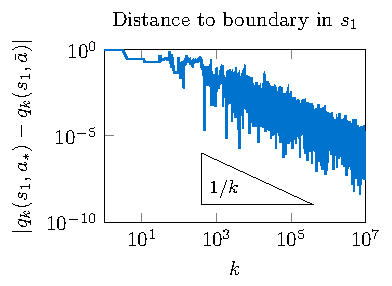
\includegraphics{figures/iv-contraction.pdf}
    %  \begin{tikzpicture}[scale=1]
    %     \begin{axis}[
    %         xmode=log,
    %         ymode=log,
    %         xlabel={$k$},
    %         ylabel={$\left|q_k(s_1,a_*)-q_k(s_1, \bar a)\right|$},
    %         grid=none,
    %         title={Distance to boundary in $s_1$},
    %         xmin=1, xmax=1e7,
    %         ymin=1e-10, ymax=1,
    %         width=0.9\linewidth,
    %         height=4.5cm,
    %     ]
    %     \addplot[
    %         CambridgeCoreBlue, line width=0.8pt
    %     ] table[
    %         x index=0,
    %         y index=1
    %     ] {figures/33/q_difference_loglog.txt};

    %     \draw[black] (axis cs:0.4*1e3,1e-9) -- (axis cs:0.4*1e6, 1e-9) -- (axis cs:0.4*1e3,1e-6) -- cycle;
    %     \node[above right, font=\small] at (axis cs:0.4*1e3, 1e-9) {$1/k$};
    %     \end{axis}
    % \end{tikzpicture}
 \end{subfigure}%
    \caption{Initial-visit MCES with sample-average updates can converge to a suboptimal solution where $q(s, a_*) = q(s, \bar a)$ for all states
    even when the greedy action is sampled at least as frequently as any other action in each state.
    % even when the sampling strategy satisfies exploring starts and the discounted MDP has stochastic transitions.
    The blue line depicts a representative solution.}
    % highlights one of ten simulations.
    % We obtain similar behaviours in states $s_2$ and $s_3$.}
    \label{fig: 3s IV ES ST}
    \vspace{-0.2cm}
\end{figure}